\documentclass[11pt,a4paper]{article}

% --- packages ---
\usepackage[a4paper, top=2cm, bottom=2cm, left=2cm, right=2cm]{geometry}
\usepackage[utf8]{inputenc}        % allow é, ï, etc.
\usepackage[T1]{fontenc}           % proper text encoding
\usepackage{tikz}                  % drawing the forest plot
\usepackage{xcolor}                % named colors
\usepackage{caption}               % \captionof{figure}{...}
\usepackage{booktabs}              % \toprule, \midrule, \bottomrule
\usepackage{graphicx}              % \includegraphics
\usepackage{eurosym}               % \euro{} for euro signs (we'll use later)
\usetikzlibrary{arrows.meta, positioning, fit}

% tighten paragraph spacing for the page budget
\setlength{\parskip}{4pt plus 1pt minus 1pt}
\setlength{\parindent}{0pt}

% figures generated by the notebook live here
\graphicspath{{reporting/figures/}}

% --- custom colors used in the figure ---
\definecolor{accent}{HTML}{2E5C8A}    % blue
\definecolor{accent2}{HTML}{4C9A4A}   % green (v3 — causally identified)
\definecolor{accent3}{HTML}{C04848}   % red (v1 — wrong sign)
\definecolor{accent4}{HTML}{E0B341}   % amber (v4, v5 — over-controlled)

\title{Dynamic Pricing for European Camping Group}
\author{Jimmy Zhang, Tobias Vanoverschelde, Fausto De Valck, Andrew Posey, 
Alexander Lievens \\ KU Leuven, Statistical Consulting 2025--2026}
\date{May 2026}

\begin{document}
\maketitle

\section{Problem and business context}

European Camping Group (ECG) operates over 400 campsites across 10 European countries, each offering several accommodation types and serving four distinct market segments. With a 30-week open season, this implies more than 250{,}000 individual prices to set every year, one for every combination of campsite, accommodation, market, and arrival-week. We refer to such a combination as a \emph{ROMGID} (reservable-option-market-group), the unit of analysis throughout the report. This project asks: can historical booking data be used to recommend better prices for these ROMGIDs, and what would that be worth in revenue?

\section{The trap}

The most direct approach, regressing booked nights on price while controlling for accommodation and seasonality, yields an answer that is economically impossible. On a 50{,}000 row training sample, the estimated price coefficient is positive: $\beta = +0.29$, with 80\% credible interval $[+0.18, +0.42]$. Read literally, this says ``raising prices increases bookings''.

The reason is structural, not statistical. ECG's pricing system already reacts to demand: when a campsite fills up, prices rise, when bookings are slow, prices fall. In the historical record, high prices and high bookings therefore tend to occur together, not because price causes bookings, but because both respond to a common, unobservable underlying demand signal.

The fix requires identifying the demand signal that the pricer reacts to. Bookings on books, the cumulative number of nights already reserved at the moment a price is set, is observed in our data and lies on the only open backdoor path between price and remaining demand. Conditioning on it blocks the reverse-causation channel and better isolates the genuine effect of price.

\begin{center}
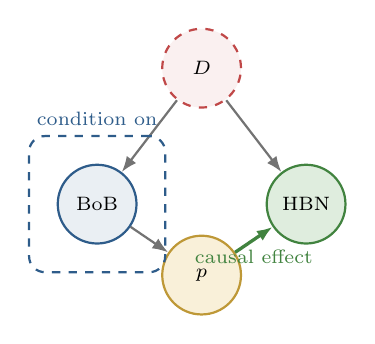
\begin{tikzpicture}[
  obs/.style={circle, draw=accent, thick, fill=accent!10, minimum size=10mm, font=\scriptsize, inner sep=0pt},
  latent/.style={circle, draw=accent3, thick, dashed, fill=accent3!8, minimum size=10mm, font=\scriptsize, inner sep=0pt},
  treatment/.style={circle, draw=accent4!85!black, thick, fill=accent4!20, minimum size=10mm, font=\scriptsize, inner sep=0pt},
  outcome/.style={circle, draw=accent2!85!black, thick, fill=accent2!18, minimum size=10mm, font=\scriptsize, inner sep=0pt},
  arrow/.style={-{Latex[length=2mm]}, thick, draw=black!55},
  causal/.style={-{Latex[length=2mm]}, thick, draw=accent2!85!black, line width=1.2pt},
]
\node[latent]    (D)                                       {$D$};
\node[obs]       (BoB) [below left=10mm and 6mm of D]      {BoB};
\node[treatment] (P)   [below=16mm of D]                   {$p$};
\node[outcome]   (Y)   [below right=10mm and 6mm of D]     {HBN};

\draw[arrow]  (D)   -- (BoB);
\draw[arrow]  (BoB) -- (P);
\draw[arrow]  (D)   -- (Y);
\draw[causal] (P)   -- (Y) node[midway, below, font=\scriptsize, color=accent2!85!black] {causal effect};

% Highlight that we condition on BoB
\node[draw=accent, thick, dashed, rounded corners=2mm, inner sep=3.5mm,
      fit=(BoB), label={[font=\scriptsize, color=accent]above:condition on}] {};
\end{tikzpicture}
\captionof{figure}{Causal structure linking price ($p$) and bookings (HBN). Latent demand $D$ (red, dashed, unobservable) drives bookings-on-books (BoB, observed) and bookings directly. The existing pricer sets $p$ in response to BoB. The path $p \leftarrow \mathrm{BoB} \leftarrow D \to \mathrm{HBN}$ is a backdoor: it lets demand contaminate the apparent price-bookings relationship. Conditioning on BoB (dashed blue box) closes it, leaving only the genuine causal effect $p \to \mathrm{HBN}$.}
\end{center}

\smallskip

\begin{center}
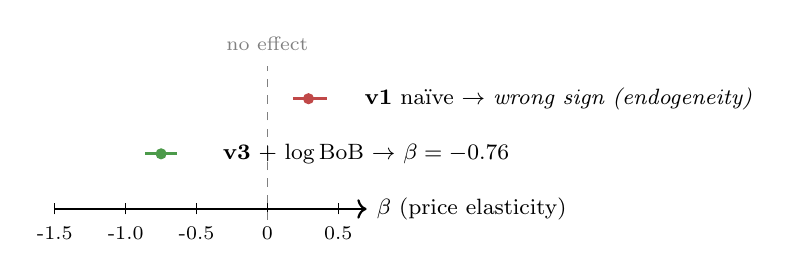
\begin{tikzpicture}[x=18mm, y=7mm]
  % axis (zoomed in to v1 / v3 range)
  \draw[->, thick] (-1.5, 0) -- (0.7, 0) node[right, font=\footnotesize] {$\beta$ (price elasticity)};
  \foreach \x in {-1.5, -1.0, -0.5, 0, 0.5} {
      \draw (\x, -0.1) -- (\x, 0.1);
      \node[below, font=\scriptsize] at (\x, -0.15) {\x};
  }
  \draw[dashed, gray] (0, -0.2) -- (0, 2.6);
  \node[gray, font=\scriptsize, above] at (0, 2.7) {no effect};

  % v1 — naïve, wrong sign
  \draw[thick, accent3, line width=1pt] (0.18, 2.0) -- (0.42, 2.0);
  \filldraw[accent3] (0.29, 2.0) circle (1.8pt);
  \node[right=3mm, font=\footnotesize] at (0.45, 2.0) {\textbf{v1} naïve $\to$ \emph{wrong sign (endogeneity)}};

  % v3 — conditioned on log_bob
  \draw[thick, accent2, line width=1pt] (-0.86, 1.0) -- (-0.64, 1.0);
  \filldraw[accent2] (-0.75, 1.0) circle (1.8pt);
  \node[right=3mm, font=\footnotesize] at (-0.55, 1.0) {\textbf{v3} $+\,\log\mathrm{BoB}$ $\to$ \emph{$\beta = -0.76$}};
\end{tikzpicture}
\captionof{figure}{Posterior point estimate and 80\% credible interval for the global price elasticity $\beta$. The naïve specification (v1) recovers an economically impossible positive sign, direct evidence of price endogeneity in ECG's data. After conditioning on bookings-on-books, the elasticity becomes negative as economic theory requires (v3, $\beta = -0.76$).}
\end{center}

\section{Two models, two jobs}

The Bayesian estimate of $\beta = -0.76$ implies demand is inelastic on average ($|\beta| < 1$). In plain language, every 1\% price increase reduces bookings by about 0.76\%. Because the response is less than proportional, total revenue (price multiplied by bookings), on average, goes up when prices go up, at least within the price range our data cover. Under a constant-elasticity assumption, this would mean ECG could raise prices uniformly and capture more revenue. A richer LightGBM optimiser in Section 4 refines this picture: average elasticity is right, but per-cell optima vary widely. Some campsite-week cells are over-priced, others under-priced, and the aggregate move is close to zero. The business case for a pricing engine on this dataset is therefore not ``raise everything'' but ``identify the asymmetries'', figuring out which cells should move, in which direction, and by how much.

v3 is intentionally minimal: only the variables strictly needed to close the backdoor. This makes it a clean estimator of the local average elasticity but not a forecaster. To predict bookings at any candidate price for any single snapshot of the booking horizon we train a gradient-boosted-trees model (LightGBM) on the same conditioning structure plus the lead-time, calendar and accommodation features that v3 deliberately omits. Trees can include all of these without the over-conditioning collapse that breaks richer Bayesian specifications. At typical prices, the LightGBM model implies the same local price-bookings slope as the Bayesian model (around $-0.75$), a useful cross-check: two methods with very different assumptions arrive at the same answer.

Out-of-sample, LightGBM achieves a median ROMGID-level error of 27\% on total booked nights, within industry norms. The error is concentrated in low-volume ROMGIDs where small absolute differences inflate percentage errors. For ROMGIDs with at least 10 bookings per season, median error drops to 22\%.

\section{The optimiser and what it recommends}

For each test-fold snapshot independently, we ask the LightGBM forecaster a counterfactual question: at this point in the booking horizon, what price would have produced the highest predicted revenue? We sweep 21 candidate price multipliers in the range $[0.85,\, 1.15] \times p_{\mathrm{obs}}$, predict bookings at each candidate, compute the implied revenue $p \cdot \hat{N}(p)$, and pick the maximum. The output for a single ROMGID is therefore not a single static price but a trajectory of 53 prices across the booking horizon, one per snapshot.

Three constraints keep the recommendation defensible: the candidate range is capped at $\pm 15\%$ of historical prices for that group, predicted bookings are clipped at capacity, and every recommendation passes through a two-tier flag (green / yellow) before deployment.

Applied to 14{,}200 ROMGIDs in the held-out test fold:

\begin{center}
\small
\begin{tabular}{@{}lr@{}}
\toprule
\textbf{Metric} & \textbf{Value} \\
\midrule
Median per-ROMGID $\Delta$price & $-0.7\%$ \\
$\Delta$price IQR (per ROMGID) & $[-6.0\%,\, +5.4\%]$ \\
\% snapshots at upper bound (1.15$\times$) & 12.7\% \\
\% snapshots at lower bound (0.85$\times$) & 14.7\% \\
\% snapshots with interior optimum & \textbf{72.6\%} \\
Total predicted uplift & \euro{}63M \\
Uplift as \% of baseline & $+38.8\%$ \\
Flag split (green / yellow) & 51\% / 49\% \\
\bottomrule
\end{tabular}
\end{center}

\begin{center}
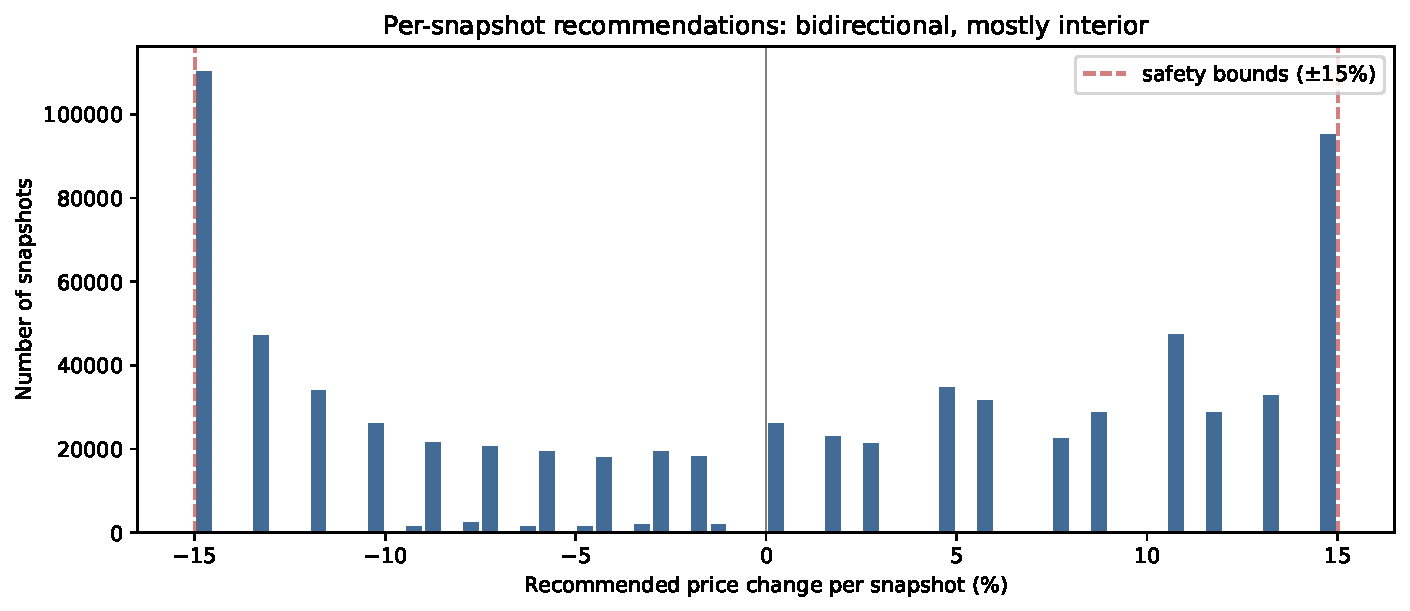
\includegraphics[width=0.7\linewidth]{recommendations_distribution.pdf}
\captionof{figure}{Distribution of recommended price changes across all test-fold snapshots. The histogram is roughly symmetric around zero, with mass at both the lower and upper safety bounds. About 73\% of decisions land at an interior optimum within the safe range, 14.7\% want a 15\% discount, and 12.7\% want a 15\% increase.}
\end{center}

The most important number on the page is the \textbf{72.6\% interior-optimum rate}. For nearly three quarters of snapshot decisions, the model finds a revenue-maximising price strictly inside the $\pm 15\%$ safe range, not at a boundary. This is something the constant-elasticity Bayesian model in Section 2 could not produce. When elasticity is forced constant the revenue function has no interior maximum, but when LightGBM learns a flexible price-demand curve, genuine interior optima emerge. The recommendations are also bidirectional, 14.7\% of snapshots want a price decrease and 12.7\% want the maximum 15\% increase. ECG is over-pricing some cells and under-pricing others, with the bulk of decisions sitting at modest interior adjustments.

\begin{center}
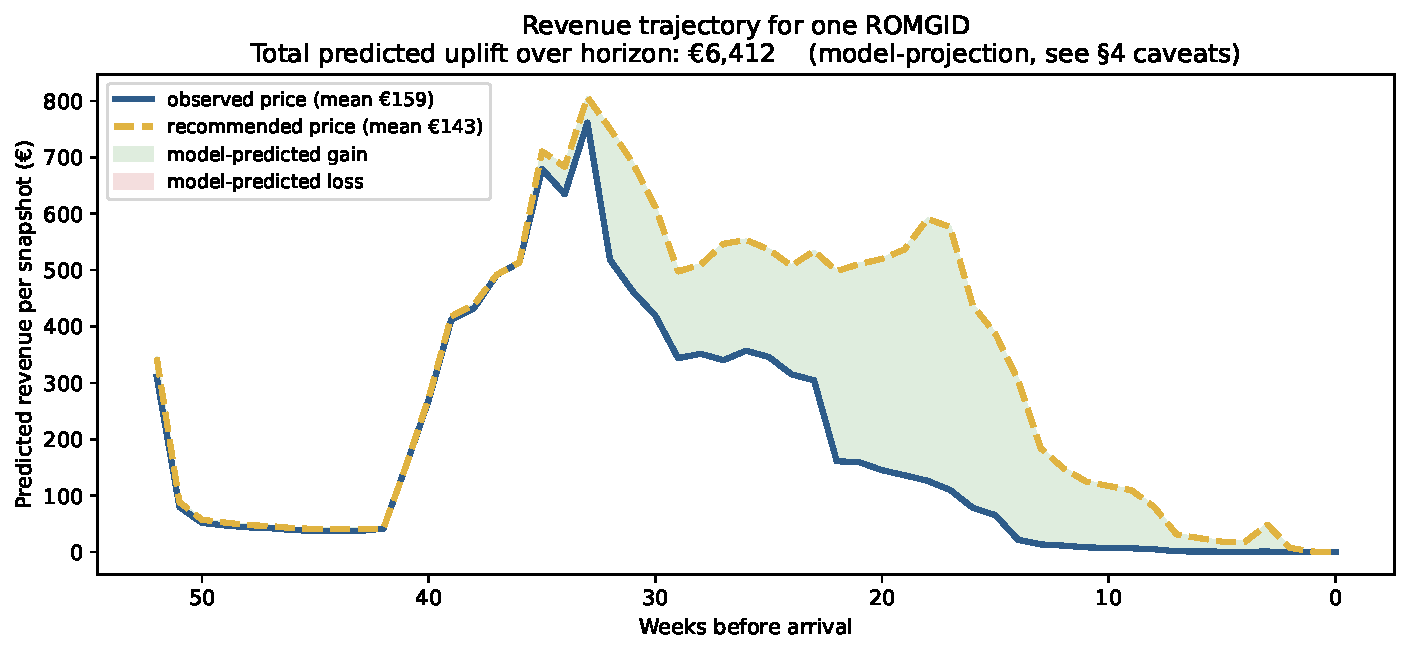
\includegraphics[width=0.7\linewidth]{revenue_trajectory.pdf}
\captionof{figure}{Predicted revenue per snapshot for one representative ROMGID, observed price (blue) versus recommended price (amber), with 80\% prediction intervals from a quantile LightGBM. Most of the booking horizon shows similar predicted revenue under both strategies, with the recommended trajectory slightly higher in the mid-horizon weeks where bookings actually concentrate.}
\end{center}

\paragraph{A fat caveat on the headline uplift.} The +\euro{}63M figure is a model projection and is almost certainly optimistic, for three reasons. First, the model has 27\% out-of-sample error on observed prices, and counterfactual prices push it further from familiar ground. Second, the optimiser picks the candidate that maximises predicted revenue, exploiting any residual model error in its own favour. Third, the model can predict small positive bookings even in late-horizon snapshots where actual bookings are essentially zero, and the optimiser sees these as small revenue gains. The directional finding (interior optima, modest adjustments, bidirectional recommendations) is robust. The magnitude is not. A randomised price experiment, discussed next, is the only way to convert it into a number ECG can budget against.

\section{What ECG should do next}

Two recommendations follow from this report, in priority order.

\paragraph{Run a small randomised price experiment.} The +\euro{}63M headline is a model projection inflated by winner's curse and noise. The only way to convert it into a number ECG can budget against is direct experimentation. Pick 100 to 200 ROMGIDs across markets and accommodation types, randomise their price by $\pm 25\%$ over a single 30-week season, and observe actual bookings. The resulting data are unbiased by the demand-autocorrelation that contaminates the historical record, and refitting the model on a mix of historical and experimental data delivers a calibrated lift estimate. The experiment also extends the recommendation envelope beyond the $\pm 15\%$ safe-range cap that currently bounds the optimiser.

\paragraph{Deploy this engine in shadow mode while improving its specification.} The recommendations have real structure: bidirectional, mostly interior, segment-differentiated. They will not be optimal in magnitude, but they identify the cells where ECG should be paying attention. Shadow-mode deployment runs the engine alongside the existing pricer for one season and lets the pricing team build trust before any auto-application. Future iterations should add better data (competitor prices, marketing-campaign indicators, the year-on-year features unavailable in this dataset) and replace the myopic per-snapshot sweep with sequential dynamic optimisation.

\paragraph{Limitations.} The methodology rests on three assumptions worth flagging. First, we close one backdoor (demand-autocorrelation via $\log\mathrm{BoB}$). Other sources of price endogeneity, such as channel-mix changes and manager overrides, remain unobservable in this dataset. Second, LightGBM's 27\% out-of-sample error grows for counterfactual prices the model has not seen, and the optimiser exploits that error in its own favour. Third, capacity is structurally non-binding here (median utilisation 10\%). A real deployment in peak weeks at premium properties would likely encounter the capacity constraint that is currently a tested but inactive safeguard.

\paragraph{Conclusion.} Treating dynamic pricing as a causal-inference problem reveals a clear endogeneity trap and a defensible local elasticity of $-0.76$ once it is closed. A complementary LightGBM forecaster delivers per-snapshot recommendations that are differentiated and bidirectional, identifying which cells should move and in which direction. The headline magnitude requires experimental validation before deployment, but the directional signal is robust enough to warrant a careful rollout. ECG's status quo is likely leaving model-identifiable revenue on the table. The size of that revenue is the open question this report cannot answer alone.


\end{document}
